
%(BEGIN_QUESTION)
% Copyright 2012, Tony R. Kuphaldt, released under the Creative Commons Attribution License (v 1.0)
% This means you may do almost anything with this work of mine, so long as you give me proper credit

A three-phase step-down transformer supplies 480 VAC to a pair of resistive loads.  The secondary winding is ``corner-grounded'' on the X2 leg:

$$\includegraphics[width=15.5cm]{i00966x01.eps}$$

Determine the following phase-to-ground voltages in this system while both loads are energized:

\begin{itemize}
\item{} $V_{G}$ = \underbar{\hskip 50pt} volts
\vskip 10pt
\item{} $V_{H}$ = \underbar{\hskip 50pt} volts
\vskip 10pt
\item{} $V_{J}$ = \underbar{\hskip 50pt} volts
\vskip 10pt
\item{} $V_{K}$ = \underbar{\hskip 50pt} volts
\vskip 10pt
\item{} $V_{L}$ = \underbar{\hskip 50pt} volts
\vskip 10pt
\item{} $V_{M}$ = \underbar{\hskip 50pt} volts
\vskip 10pt
\item{} $V_{N}$ = \underbar{\hskip 50pt} volts
\end{itemize}

Supposing the upper load has a total power dissipation of 8.4 kW and the lower load has a total power dissipation of 3.9 kW, calculate the amount of current through line H2.

\underbar{file i00966}
%(END_QUESTION)





%(BEGIN_ANSWER)

\begin{itemize}
\item{} $V_{G}$ = 0 volts
\vskip 10pt
\item{} $V_{H}$ = 480 volts
\vskip 10pt
\item{} $V_{J}$ =  volts
\vskip 10pt
\item{} $V_{K}$ = 480 volts
\vskip 10pt
\item{} $V_{L}$ = 0 volts
\vskip 10pt
\item{} $V_{M}$ = 480 volts
\vskip 10pt
\item{} $V_{N}$ = 480 volts
\end{itemize}

The phase-to-ground voltage at point J must be calculated trigonometrically:

$$\includegraphics[width=15.5cm]{i00966x02.eps}$$

Each interior angle of the triangle GHK is 60$^{o}$.  Angle JGK is 30$^{o}$.  Angle GJK is 120$^{o}$.  Phasor JK's length may be calculated using the Law of Sines, where the ratio of side length to the sine of the opposite angle is constant for {\it any} triangle:

$${A \over \sin a} = {B \over \sin b}$$

$${480 \over \sin 120} = {V_{JK} \over \sin 30}$$

$$V_{JK} = \sin 30 \left({480 \over \sin 120}\right)$$

$$V_{JK} = 0.5 \left({480 \over 0.866}\right)$$

$$V_{JK} = 277.13 \hbox{ volts}$$

\filbreak

Total power in this system is 12.3 kW.  The line current at the primary side of the transformer (assuming no power losses in the transformer) may be calculated as follows:

$$P_{total} = \sqrt{3} (I_{line}) (V_{line})$$

$$I_{line} = {P_{total} \over \sqrt{3} (V_{line})}$$

$$I_{line} = {12300 \over \sqrt{3} (13800)}$$

$$I_{line} = 0.5146 \hbox{ amps}$$

The grounding of the secondary is irrelevant to calculations of current and power, because that ground connection conducts no current at all and dissipates no power.

%(END_ANSWER)





%(BEGIN_NOTES)


%INDEX% Electronics review: 3-phase voltage/current/power calculation

%(END_NOTES)


